\documentclass[aspectratio=169,10pt]{beamer}
\usepackage[T1]{fontenc}
\usepackage[utf8]{inputenc}
\usepackage{booktabs,tikz}
\usepackage{helvet}
\renewcommand{\familydefault}{\sfdefault}
\usetikzlibrary{arrows.meta,positioning}
\usetheme{Madrid}
\definecolor{ink}{HTML}{142C43}
\definecolor{accent}{HTML}{007F86}
\setbeamercolor{structure}{fg=accent}
\setbeamercolor{frametitle}{bg=ink,fg=white}
\setbeamercolor{title}{bg=ink,fg=white}
\setbeamertemplate{navigation symbols}{}
\setbeamertemplate{footline}{\hfill\scriptsize Soliton Microcombs\quad |\quad October 2026\quad |\quad\insertframenumber\hspace{5mm}\vspace{3mm}}
\newcommand{\status}[1]{\par\vspace{2mm}{\scriptsize\color{accent}#1\par}}
\newcommand{\source}[2]{\vfill{\tiny Source: \href{#1}{#2}}}
\title{Soliton Microcombs}
\subtitle{Multi-wavelength light sources for optical interconnects}
\author{Pavel Chekmaryov}
\institute{\href{mailto:p@occurai.com}{p@occurai.com}}
\date{October 2026}
\begin{document}

\begin{frame}
\titlepage
\centering\large One pump. Many optical carriers.\\[3mm]
\normalsize\textbf{\$750k pre-seed}\quad |\quad 15-month feasibility program
\end{frame}

\begin{frame}{The Problem: Light Sources for Optical Interconnects}
\begin{block}{The customer}
Optical interconnects need several stable wavelengths of light. The light source must provide enough power on each wavelength without making the system too expensive or power-hungry.
\end{block}
\begin{itemize}
\item Existing laser modules already provide several wavelengths across multiple fibers.
\item Adding more wavelengths can make control, packaging, and testing harder.
\item Our source must meet the customer's requirements and offer a measurable cost or power advantage.
\end{itemize}
\begin{exampleblock}{Our opportunity}
Use one pump laser and a microcomb chip to generate many wavelengths in a compact module.
\end{exampleblock}
\source{https://ayarlabs.com/supernova}{Ayar Labs: SuperNova multi-wavelength, multi-port source}
\end{frame}

\begin{frame}{Our Solution: One Pump Laser, Many Wavelengths}
\centering
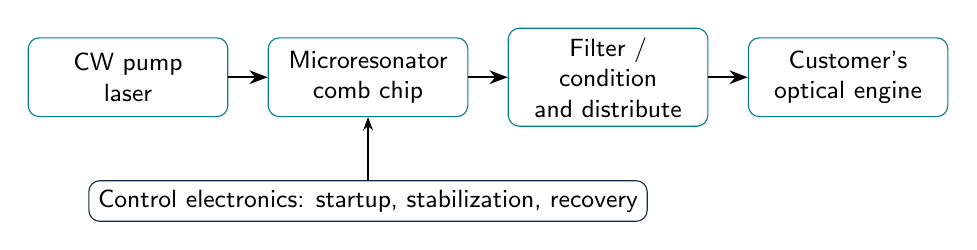
\begin{tikzpicture}[node distance=5mm,box/.style={draw=accent,rounded corners,align=center,text width=2.3cm,minimum height=1.0cm,font=\small},>=Stealth]
\node[box] (pump) {CW pump\\laser};
\node[box,right=of pump] (comb) {Microresonator\\comb chip};
\node[box,right=of comb] (out) {Filter / condition\\and distribute};
\node[box,right=of out] (host) {Customer's\\optical engine};
\draw[->,thick] (pump)--(comb);
\draw[->,thick] (comb)--(out);
\draw[->,thick] (out)--(host);
\node[draw=ink,rounded corners,below=8mm of comb,align=center,font=\small] (control) {Control electronics: startup, stabilization, recovery};
\draw[->] (control)--(comb);
\end{tikzpicture}
\vspace{5mm}
\begin{itemize}
\item Gen 1 uses an external pump and established foundry processes.
\item The module includes filters and control electronics, plus amplification if needed.
\item The customer keeps their modulators and receivers. We test whether our source works with them.
\end{itemize}
\status{Development objective. Packaged performance and manufacturing cost remain to be validated.}
\end{frame}

\begin{frame}{What We Will Build with This Round}
\begin{columns}[T]
\begin{column}{.48\textwidth}
\begin{block}{Starting point}
\begin{itemize}
\item Chip design and simulations led by the founder.
\item Scientific guidance on semiconductor optics and practical fabrication.
\item No measured module performance or signed customer commitment is claimed in this deck.
\end{itemize}
\end{block}
\end{column}
\begin{column}{.48\textwidth}
\begin{exampleblock}{What we will demonstrate}
\begin{itemize}
\item A fabricated chip with usable wavelengths measured at the output.
\item Automated startup, stabilization, and recovery.
\item Measured module power and an estimate of manufacturing cost.
\item Testing by an outside lab or potential customer against agreed requirements.
\end{itemize}
\end{exampleblock}
\end{column}
\end{columns}
\vspace{3mm}
\textbf{First prototype target:} 16 usable carriers at an agreed band, grid, and delivered per-line power.\\[2mm]
\textbf{Next target:} 32--50 usable carriers, subject to optical budget and customer need.
\end{frame}

\begin{frame}{Performance and Cost: What We Need to Measure}
\begin{tabular}{p{.24\textwidth}p{.32\textwidth}p{.32\textwidth}}
\toprule
\textbf{Comparison} & \textbf{What we compare} & \textbf{How we check}\\
\midrule
Customer cost & Module price at the same useful wavelength count and output power & Customer baseline and supplier quotes\\[2mm]
Electrical power & Pump, controls, thermal management, amplification & Wall-plug measurement\\[2mm]
Optical quality & Delivered line power, noise, grid accuracy & Spectrum and transmission results\\[2mm]
Reliability & Startup, drift, recovery, operating conditions & Defined test protocol\\
\bottomrule
\end{tabular}
\begin{block}{Production cost targets}
At 2,500 modules/year: \textbf{\$3,500 selling price}, \textbf{\$1,575 manufacturing cost}, \textbf{55\% gross margin}. These are assumptions to validate, not quoted costs.
\end{block}
\status{We will measure the improvement against an existing module with the same output requirements.}
\end{frame}

\begin{frame}{Competition and Our Advantage}
\begin{itemize}
\item \textbf{Ayar SuperNova:} up to 16 wavelengths per fiber across 16 fibers; an established optical-I/O source alternative.
\item \textbf{Lightmatter Guide:} up to 16 wavelengths per fiber, 16 output fibers, 200 GHz grid.
\item \textbf{Other approaches:} integrated laser arrays, other comb architectures, and internal source development.
\end{itemize}
\begin{exampleblock}{What we aim to improve}
Lower cost for the required number of wavelengths; reliable automatic operation; repeatable manufacturing; and compatibility with the customer's system.
\end{exampleblock}
\textbf{Our IP:} develop and protect new chip designs and control methods where they offer an advantage over existing work.
\status{These companies are possible customers or competitors. No partnership is claimed.}
\source{https://lightmatter.co/wp-content/uploads/2025/08/57-lightmatter_hotchips_2025_final.pdf}{Lightmatter, Hot Chips 2025, slide 17; Ayar Labs SuperNova product page}
\end{frame}

\begin{frame}{Go-to-Market Strategy}
\begin{enumerate}
\item \textbf{Specify:} obtain wavelength band/grid, delivered power, noise, port count, and reliability requirements from prospects.
\item \textbf{Evaluate:} supply lab prototypes and collect performance data against those requirements.
\item \textbf{Design in:} agree integration responsibilities, qualification criteria, and commercial terms.
\item \textbf{Ship:} qualify the module, deliver low-rate orders, then ramp with the customer's system program.
\end{enumerate}
\begin{block}{How we make money}
Sell packaged modules. Start with paid test samples, then production orders after customer testing and approval.
\end{block}
\status{Planning: evaluations in Year 2, low-rate shipments in Year 3, meaningful ramp in Years 4--7. Qualification timing remains customer-dependent.}
\end{frame}

\begin{frame}{Market Opportunity}
\begin{block}{Initial market}
Companies building optical interconnects for data centers and AI systems. We initially sell to the companies designing the optical hardware, which supplies the larger systems.
\end{block}
\centering\large
Annual system shipments $\times$ modules/system $\times$ module ASP\\[3mm]
\normalsize yields the annual source opportunity in each qualified segment.
\begin{exampleblock}{Year 5 sales assumption}
Year 5: five shipping programs averaging 500 modules/year = \textbf{2,500 modules}.\\
At \$3,500/module, this supports \textbf{\$8.75M annual product revenue}.
\end{exampleblock}
\textbf{Long-term sales goal:} a \$100M annual business requires roughly 33,300 modules at a \$3,000 ASP, across multiple production programs.
\status{Program counts and volumes are assumptions. Account-level validation is required; no unsupported headline TAM is used.}
\end{frame}

\begin{frame}{Revenue Projections}
\centering
\begin{tabular}{lrrrr}
\toprule
\textbf{Annual product revenue} & \textbf{Y2} & \textbf{Y3} & \textbf{Y5} & \textbf{Y7}\\
\midrule
Delayed adoption & \$0 & \$0.135M & \$1.75M & \$10.5M\\
Base case & \$0.10M & \$0.675M & \$8.75M & \$36.0M\\
Upside & \$0.20M & \$1.350M & \$24.5M & \$105.0M\\
\bottomrule
\end{tabular}
\vspace{4mm}
\begin{itemize}
\item Base volume: 20 modules in Y2; 150 in Y3; 2,500 in Y5; 12,000 in Y7.
\item Selling price declines from \$5,000 for evaluation modules toward \$3,000 at scale.
\item Gross-margin targets progress from 20\% early to 55\% in Y5 and 60\% in Y7.
\item Licensing, grants, and acquisition proceeds are excluded from operating revenue.
\end{itemize}
\status{Illustrative scenarios in USD; years start at financing close. These are not contracted demand or probability-weighted forecasts. Technical failure can produce zero revenue.}
\end{frame}

\begin{frame}{15-Month Development Roadmap}
\begin{tabular}{p{.15\textwidth}p{.71\textwidth}}
\toprule
\textbf{Window} & \textbf{Milestones}\\
\midrule
M0--3 & Technical lead; fabrication, packaging, and lab quotes; requirements from two potential customers; wavelength band and spacing selected.\\[2mm]
M3--6 & Tapeout and test plan; characterized process structures as fabrication timing permits.\\[2mm]
M6--9 & Comb generation; delivered usable-line spectrum; measured optical and electrical power.\\[2mm]
M9--12 & Automated lab prototype; proposed tests: 24-hour operation and 95 successful cold starts in 100 attempts under defined conditions.\\[2mm]
M12--15 & External lab evaluation; integration requirements and next design cycle defined; partner-supported transmission test if equipment access permits.\\
\bottomrule
\end{tabular}
\status{Targets depend on quotes, turnaround, and lab access. Begin follow-on fundraising around M8--10; allow contingency for a failed first fabrication.}
\end{frame}

\begin{frame}{Team and Who We Are Looking For}
\begin{block}{Pavel Chekmaryov --- Founder}
Hardware/software experience, including Snowcap Compute; technical recruitment, early-stage startup operations, product development, and growth.
\end{block}
\begin{block}{Scientific guidance}
Anton Velichko (University of Sheffield): semiconductor optics, AlGaAs, and fabrication-aware design. Scope of engagement and public attribution to be confirmed.
\end{block}
\begin{exampleblock}{Seeking a technical co-founder or photonics engineer}
Someone with hands-on experience in microresonators, comb generation, chip fabrication, packaging, and optical testing.
\end{exampleblock}
\textbf{How we keep costs manageable:} a small team, specialist help when needed, and shared lab and test equipment.
\end{frame}

\begin{frame}{Funding Ask: \$750k Pre-Seed}
\begin{columns}[T]
\begin{column}{.47\textwidth}
\begin{tabular}{lr}
\toprule
\textbf{15-month allocation} & \textbf{USD}\\
\midrule
People / specialist support & \$250k\\
Fabrication / packaging & \$220k\\
Lab / test access & \$100k\\
Operations / IP & \$65k\\
Contingency & \$115k\\
\midrule
\textbf{Total} & \textbf{\$750k}\\
\bottomrule
\end{tabular}
\end{column}
\begin{column}{.49\textwidth}
\begin{exampleblock}{What this round buys}
A working lab prototype with automatic control, measured power and wavelength output, a manufacturing cost estimate, and outside testing.
\end{exampleblock}
\textbf{Next round:} fund customer approval and initial production. Our base-case plan allows roughly \$9--12M in total funding, including this round; the amount depends on testing and production costs.
\end{column}
\end{columns}
\vspace{4mm}
\textbf{Our goal:} build a business selling light-source modules. Acquisition is a possible outcome, but we do not assume a buyer, date, or price.
\status{Budget assumes shared lab/test access and lean staffing; supplier quotes remain necessary.}
\end{frame}

\appendix
\begin{frame}{Appendix: acceptance specification and optical budget}
\begin{itemize}
\item Define band, spacing, port count, per-line delivered power, flatness, noise, operating temperature, and recovery behavior before finalizing the design.
\item Count \emph{usable} carriers at the customer's interface, not visible spectrum peaks.
\item Measure the full electrical system, including pump, thermal control, filtering, electronics, and amplification where required.
\end{itemize}
\begin{block}{Illustrative power constraint}
64 carriers $\times$ 1 mW delivered = 64 mW output.\\
At 5\% usable pump-to-comb efficiency and 50\% transmission: 2.56 W optical pump.\\
At 20\% pump wall-plug efficiency: 12.8 W electrical, before controls.\\
Multi-port fan-out increases the demand if each port needs the same power.
\end{block}
\status{Example assumptions, not our measured performance. A 1 W module claim requires a demonstrated efficiency and link budget.}
\source{https://www.nature.com/articles/s44310-024-00030-9}{Review of Kerr microcomb conversion efficiency}
\end{frame}

\begin{frame}{Appendix: band compatibility and data demonstration}
\begin{itemize}
\item Lightmatter's published Guide spectrum is in the O-band; a C-band comb is not automatically compatible with that source interface.
\item Foundry selection must support the required dispersion, operating band, coupling, and thermal tuning.
\item Start with external pump and modular test equipment; heterogeneous integration follows demonstrated economics and performance.
\end{itemize}
\begin{exampleblock}{Transmission evidence}
Document modulation, rate/channel, simultaneous usable channels, BER, FEC, receiver, losses, run duration, and temperature.\\[2mm]
Example: 40 channels $\times$ 25 Gb/s = 1 Tb/s gross aggregate. This is a possible later demonstration, not a guaranteed deliverable of the lean raise.
\end{exampleblock}
\source{https://lightmatter.co/wp-content/uploads/2025/08/57-lightmatter_hotchips_2025_final.pdf}{Lightmatter, Hot Chips 2025, slide 17}
\end{frame}

\begin{frame}{Appendix: base-case costs and cash requirements}
\centering\small
\begin{tabular}{lrrrrr}
\toprule
 & \textbf{Y1} & \textbf{Y2} & \textbf{Y3} & \textbf{Y5} & \textbf{Y7}\\
\midrule
Modules & 0 & 20 & 150 & 2,500 & 12,000\\
ASP & \$5,000 & \$5,000 & \$4,500 & \$3,500 & \$3,000\\
COGS / module & \$4,000 & \$4,000 & \$3,000 & \$1,575 & \$1,200\\
Product revenue (\$M) & 0 & .100 & .675 & 8.750 & 36.000\\
Cash opex (\$M) & .350 & .850 & 1.600 & 4.500 & 10.000\\
Capex (\$M) & .100 & .150 & .250 & .600 & 1.000\\
\bottomrule
\end{tabular}
\vspace{4mm}
\begin{itemize}
\item Delivered COGS must include yield loss, pump/conditioning, assembly, test, and warranty allowances.
\item Working capital is provisionally 20\% of revenue; replace with inventory, deposits, receivables, and payables.
\item Annual cash flows omit intra-year troughs, tax, financing costs, and reserve. The provisional \$9--12M envelope requires a monthly qualification/production plan.
\end{itemize}
\status{Month-by-month pre-seed budget and editable seven-year model accompany this deck. Cost learning is assumed, not established.}
\end{frame}

\begin{frame}{Appendix: investor-return sensitivity, not an exit forecast}
\textbf{Illustration:} \$750k at an \$8M post-money cap.\\
After dilution, 60\% of initial ownership remains: 5.625\% at exit.
\par
\vspace{4mm}
\centering
\begin{tabular}{rrr}
\toprule
\textbf{Exit equity value} & \textbf{Gross proceeds} & \textbf{Gross multiple}\\
\midrule
\$50M & \$2.81M & 3.75x\\
\$100M & \$5.63M & 7.50x\\
\$200M & \$11.25M & 15.00x\\
\$300M & \$16.88M & 22.50x\\
\$500M & \$28.13M & 37.50x\\
\bottomrule
\end{tabular}
\par
\vspace{4mm}
\raggedright
Actual returns depend on entry terms, dilution, liquidation preferences, debt, and exit equity proceeds. This simplified cap-binding illustration excludes additional investment, fees, and taxes. No exit probability or timing is assumed.
\status{The cap is a sensitivity input, not an offered financing term. Failure can return zero.}
\end{frame}

\begin{frame}{Future Application: Photonic Retina}
\begin{block}{The idea}
Combine optical sensing with photonic processing, so a sensor can extract useful features close to where it captures the image.
\end{block}
\centering
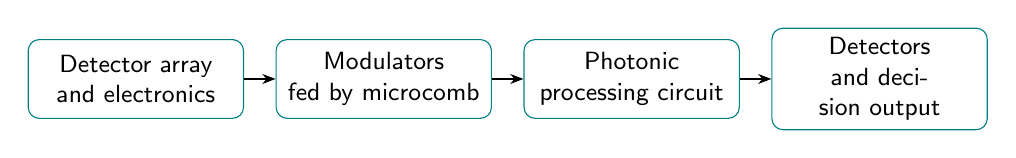
\begin{tikzpicture}[node distance=4mm,box/.style={draw=accent,rounded corners,align=center,text width=2.5cm,minimum height=1cm,font=\small},>=Stealth]
\node[box] (sense) {Detector array\\and electronics};
\node[box,right=of sense] (encode) {Modulators\\fed by microcomb};
\node[box,right=of encode] (process) {Photonic\\processing circuit};
\node[box,right=of process] (read) {Detectors\\and decision output};
\draw[->] (sense)--(encode); \draw[->] (encode)--(process); \draw[->] (process)--(read);
\end{tikzpicture}
\vspace{3mm}
\begin{itemize}
\item \textbf{First experiment:} a small detector array and a simple task, such as detecting whether a bright object is on the left or right.
\item \textbf{What to measure:} accuracy, total power, and time from sensing to result, compared with an electronic setup performing the same task.
\item \textbf{Role of the comb:} test whether several wavelengths help process inputs in parallel enough to justify the added hardware.
\end{itemize}
\status{Possible future application, outside the current budget and revenue projections. This setup includes electrical sensing and modulation; performance remains to be tested.}
\source{https://www.nature.com/articles/s41586-022-04714-0}{Related work: on-chip photonic image classification, Nature (2022); a different architecture}
\end{frame}

\begin{frame}{Long-Term Vision: Hopfion Computing}
\begin{block}{From light sources to photonic computing}
Experience with light sources, control, and packaging could help us explore interconnected photonic systems and new ways to process information.
\end{block}
\begin{itemize}
\item \textbf{Hopfions:} explore whether linked three-dimensional structures of light can be used to store or process information.
\item \textbf{First steps:} model the system, create and measure the optical structure, then test whether it can perform a useful task.
\item \textbf{Further direction:} investigate connected resonators and Hopf-fibration-inspired architectures if the experiments show useful behavior.
\end{itemize}
\status{Long-term research, outside this raise. No compute-product date or revenue is assumed; future experiments need their own funding.}
\source{https://www.nature.com/articles/s41467-021-26171-5}{Particle-like topologies in light, Nature Communications (2021)}
\end{frame}

\begin{frame}{Appendix: evidence and references}
\small
\begin{itemize}
\item \href{https://ayarlabs.com/supernova}{Ayar Labs: SuperNova product specifications}.
\item \href{https://lightmatter.co/wp-content/uploads/2025/08/57-lightmatter_hotchips_2025_final.pdf}{Lightmatter: Hot Chips 2025, Guide source (slide 17)}.
\item \href{https://www.nature.com/articles/s44310-024-00030-9}{Kerr microcomb conversion-efficiency review (2024)}.
\item \href{https://arxiv.org/abs/1911.02636}{Integrated turnkey soliton microcombs operated at CMOS frequencies}.
\item \href{https://www.nature.com/articles/s41467-021-26171-5}{Particle-like topologies in light (2021)}.
\end{itemize}
\begin{block}{Company-specific evidence to complete}
Measured prototype data; foundry and packaging quotations; customer specifications/evaluation status; technical-lead commitment; advisor attribution; and design/control IP ownership.
\end{block}
\status{External publications establish context, not company traction or achieved performance. All financial figures are USD planning assumptions.}
\end{frame}
\end{document}
